%=======================================================================
% File         : urt_setup.tex
% Author(s)    : Sebastien VARRETTE <Sebastien.Varrette@uni.lu>
% Creation     : 06 Jul 2009
% Time-stamp:    <Thu 2012-07-26 11:39 svarrette>
%  
%   Copyright (c) 2009 Sebastien Varrette. 
%
% Licence: Creative Commons Attribution-Noncommercial-Share Alike 2.0 France
%
% You are free:
%   - to Share:  to copy, distribute and transmit the work
%   - to Remix: to adapt the work
%
% Under the following conditions:
%   - Attribution : You must attribute the work in the manner specified by the
%                   author or licensor (but  not in any way that suggests that
%                   they endorse you or your use of the work).  
%   - Noncommercial:  You may not use this work for commercial purposes.
%   - Share Alike: If you alter, transform, or build upon this work, you may
%                  distribute the resulting work only under the same or similar
%                  license to this one. 
%
% With the understanding that:
%   - Waiver: Any of the above conditions can be waived if you get permission from
%             the copyright holder. 
%   - Other Rights: In no way are any of the following rights affected by the
%                   license:  
%                    * Your fair dealing or fair use rights;
%                    * Apart from the remix rights granted under this license,
%                      the author's moral rights; 
%                     * Rights other persons may have either in the work itself
%                       or in how the work is used, such as publicity or privacy
%                       rights. 
%   - Notice:  For any reuse or distribution, you must make clear to others the
%              license terms of this work. The best way to do this is with a
%              link to this web page. 
%=======================================================================

\documentclass[11pt,twoside,a4paper]{article}
%--- Package insertion ---
\usepackage{ae,a4,url}
\usepackage[T1]{fontenc}
\usepackage{epsfig}
%\usepackage{hevea}
\usepackage{hyperref}
\usepackage{graphicx}
\usepackage{amsmath, amsthm}
\usepackage{amsfonts,amssymb} % permet la definition des ensembles
\usepackage{float}
\usepackage{acronym}             % for acronyms
\usepackage{multirow}             

%%%%%%%%%%%%%%%%%%%%%%%%%%%%%%%%%%%%%%%%
% Versionning with day and time
%%%%%%%%%%%%%%
% months
\def\ftoday{\number\day\space
 \ifcase\month\or
 january\or february\or march\or april\or may\or june\or
 july\or august\or september\or october\or november\or december\fi
 \space\number\year}
% \isodayandtime to get current date and time
\begingroup
\count0=\time \divide\count0by60 % Hour
\count2=\count0 \multiply\count2by-60 \advance\count2by\time% Min
\def\2#1{\ifnum#1<10 0\fi\the#1}
\xdef\isodayandtime{\the\year-\2\month-\2\day\space\2{\count0}:%sec
\2{\count2}}
\endgroup


%%%%%%%%%%%%%%%%%%%%%%%%%%%%%%%%%%%%%%%%
% Code Listings
%%%%%%%%%%%%%%
\usepackage[usenames]{color}
\usepackage{xspace}
\usepackage{listings}
\definecolor{bcode}{rgb}{0.9,0.9,0.9} % font color for the listings
% default style
\lstset{numbers=left,numberstyle=\tiny,stepnumber=3,firstnumber=1,language=C++,basicstyle=\small,columns=flexible,backgroundcolor=\color{bcode},showstringspaces=false,escapeinside={/*@}{@*/}}
% specific styles
\lstdefinestyle{filecontent}
{language=sh,emph={remoteSite,mySite,remoteserver,password_remoteSite,remoteSiteID},emphstyle=\itshape,numbers=none,commentstyle={},columns=flexible}
\lstdefinestyle{command}
{language=sh,emph={user@host,root@host},emphstyle=\textbf,numbers=none,commentstyle={},columns=flexible}
\lstdefinestyle{urtcfg}
{language=sh,emph={sets,set},emphstyle=\textbf,morecomment=[l]{//},numbers=none,columns=flexible}
\lstdefinestyle{apachecfg}
{language=sh,emph={NameVirtualHost,ServerAdmin,ServerName,Directory,VirtualHost,IfModule},emphstyle=\textbf,basicstyle=\footnotesize,numbers=none}

\newcommand{\mybox}  [1]{\colorbox{bcode}{\makebox[\linewidth][l]{#1}}}
\newcommand{\prompt} [5]{{\small \mybox{\texttt{[#1@#2]}#3\texttt{#4 #5}}}}
\newcommand{\cmd}    [1]{{\small \mybox{~~\texttt{#1}}}}
\newcommand{\cmdres} [1]{{\small \mybox{~~#1}}}
\newcommand{\install}[1]{\texttt{apt-get install #1}}
\newcommand{\promptRS}[2]{\prompt{root}{server}{#1}{\#}{#2}}
\newcommand{\promptUS}[2]{\prompt{user}{server}{#1}{\$}{#2}}
\newcommand{\promptRH}[2]{\prompt{root}{host}{#1}{\#}{#2}}
\newcommand{\promptUH}[2]{\prompt{user}{host}{#1}{\$}{#2}}

\newcommand{\begginstall}{\texttt{\$B3\_EGG\_INSTALLDIR}}
\newcommand{\bhome}{\texttt{\$B3\_HOMEDIR}}
\newcommand{\bconf}{\texttt{\$B3\_CONFDIR}}
\newcommand{\bextplugins}{\texttt{\$B3\_EXTPLUGINSDIR}}


% Logos 
\newcommand{\windows}{
\includegraphics[height=1em]{Images/logo_windows_small.jpg}}
\newcommand{\linux}  {
\includegraphics[height=1em]{Images/logo_linux_small.jpg}}
\newcommand{\macosx} {
\includegraphics[height=1em]{Images/logo_apple_small.jpg}}

% separators
\newcommand{\setitemsep}{\setlength{\itemsep}{-0.3ex}}


\bibliographystyle{plain}


%%%%%%%%%%%%%%%%%%%%%%%%%%%%%%%%%%%%%%%
%%%%%%%%%%%%%%%%%%%%%%%%%%%%%%%%%%%%%%%

\title{
  {\rule{\textwidth}{1mm}}\\[1em]
  \textsc{Urban Terror [Server] Guide}\\[0.75em]
  {\rule{\textwidth}{1mm}}  
}
\author{Sebastien Varrette\\ {\small \url{Sebastien.Varrette@uni.lu}}}

\date{Version 0.3.0-b8\thanks{Draft version. Compiled time: \isodayandtime}}

\begin{document}
\maketitle

\begin{abstract}
  This tutorial details the configuration of a Linux server for Urban Terror
  (UrT~\cite{urt}), a free multiplayer first person shooter (FPS) based on the
  Quake 3 engine~\cite{ioq3}.  Urban Terror is very similar to CounterStrike and
  can be described as a Hollywood tactical shooter. Yet UrT is cross-platform
  meaning the software package exists for Windows, Linux and Mac OS X.

  Whereas everybody can start a server from the client software, such approach
  does not authorize votes during the game, or statistics.  Consequently, it is
  better to setup the server on a dedicated machine, as proposed in this document.
  In particular, apart from the UrT server setup, this tutorial details the
  installation of BigBrotherBot (B3)~\cite{b3}, a complete and total server
  administration package for online games (including UrT) and various plugins (for
  player statistics etc.).

  The latest version of this tutorial (together with the \LaTeX\ sources of the
  document) are freely available on
  \href{https://github.com/Falkor/urbanterror_guide}{GitHub} at the following
  address:
  \begin{center}
       \url{https://github.com/Falkor/urbanterror_guide}.
  \end{center}
\end{abstract}

\clearpage
~\vfill
%=======================================================================
% File         : _licence.tex
% Title        :  Creative Commons Licence
% Author(s)    : Sebastien VARRETTE <Sebastien.Varrette@uni.lu>
% Creation     : 06 Jul 2009
% Time-stamp:    <2009-07-06 16:15:53 svarrette>
%=======================================================================

\paragraph{Licence: Creative Commons 2.0.}

{\footnotesize
This document is released under the terms of the CC licence Creative Commons \emph{Attribution-Noncommercial-Share Alike} 2.0 France.

\noindent You are free:
\begin{itemize}
\item \textbf{to Share} -- to copy, distribute and transmit the work
\item \textbf{to Remix} -- to adapt the work
\end{itemize}

\noindent Under the following conditions:
\begin{itemize}
\item \textbf{Attribution} -- You must attribute the work in the manner specified by the author or
  licensor (but not in any way that suggests that they endorse you or your use of the work).
\item \textbf{Noncommercial} -- You may not use this work for commercial purposes.
\item \textbf{Share Alike} -- If you alter, transform, or build upon this work, you may distribute
  the resulting work only under the same or similar license to this one.
\end{itemize}

\noindent With the understanding that:
\begin{itemize}
\item \textbf{Waiver} -- Any of the above conditions can be waived if you get permission from the
  copyright holder.
\item \textbf{Other Rights} -- In no way are any of the following rights affected by the license:
  \begin{itemize}
  \item Your fair dealing or fair use rights;
  \item Apart from the remix rights granted under this license,
    the author's moral rights;
  \item Rights other persons may have either in the work itself or in how the
    work is used, such as publicity or privacy rights.
  \end{itemize}

\item \textbf{Notice} -- For any reuse or distribution, you must make clear to others the license terms of this work. The best way to do this is with a link to this web page.
\end{itemize}

}



%~~~~~~~~~~~~~~~~~~~~~~~~~~~~~~~~~~~~~~~~~~~~~~~~~~~~~~~~~~~~~~~~
% eof
%
% Local Variables:
% fill-column: 100
% mode: latex
% mode: flyspell
% End:

\clearpage

\tableofcontents
\clearpage


%==========================
\section{Introduction}
\label{sec:intro}
%=======================================================================
% File         : _intro.tex
% Title        : 
% Author(s)    : Sebastien VARRETTE <Sebastien.Varrette@uni.lu>
% Creation     : 06 Jul 2009
% Time-stamp:    <Thu 2012-07-26 11:34 svarrette>
%  
%   Copyright (c) 2009 Sebastien Varrette. 
%
% Licence: Creative Commons Attribution-Noncommercial-Share Alike 2.0 France
%
% You are free:
%   - to Share:  to copy, distribute and transmit the work
%   - to Remix: to adapt the work
%
% Under the following conditions:
%   - Attribution : You must attribute the work in the manner specified by the
%                   author or licensor (but  not in any way that suggests that
%                   they endorse you or your use of the work).  
%   - Noncommercial:  You may not use this work for commercial purposes.
%   - Share Alike: If you alter, transform, or build upon this work, you may
%                  distribute the resulting work only under the same or similar
%                  license to this one. 
%
% With the understanding that:
%   - Waiver: Any of the above conditions can be waived if you get permission from
%             the copyright holder. 
%   - Other Rights: In no way are any of the following rights affected by the
%                   license:  
%                    * Your fair dealing or fair use rights;
%                    * Apart from the remix rights granted under this license,
%                      the author's moral rights; 
%                     * Rights other persons may have either in the work itself
%                       or in how the work is used, such as publicity or privacy
%                       rights. 
%   - Notice:  For any reuse or distribution, you must make clear to others the
%              license terms of this work. The best way to do this is with a
%              link to this web page. 
%=======================================================================

Urban Terror (UrT for short) started as a realism mod for Quake III Arena,
reusing most of the concepts of the famous game Counterstrike~\cite{cs}.
The approach is similar to the one proposed by the Tactical Ops\footnote{See
\url{http://www.tactical-ops.de/}} mod for Unreal Tournament.
Yet with the release of the Quake III engine as an open-source software (through
the \texttt{ioquake3} project~\cite{ioq3}), Urban Terror is now completely free,
stand-alone (\emph{i.e.} it does not require to buy a copy of Quake III Arena)
and, more importantly, cross-platform so it can run on Windows \windows, Linux
\linux\ and Mac OS X \macosx.    
\\
The software package in itself comes with two elements: 
\begin{enumerate}\setitemsep
\item the client executable \texttt{ioUrbanTerror} for playing on a remote
  dedicated server. It is also possible to start a server at the same time you
  play to host a game and let other player join your game other the network;
\item a dedicated server executable \texttt{ioUrTded}.
\end{enumerate}

Whereas the UrT client can start a server, you have  access in this case to
limited functionality (in particular no votes) and performances (as your machine
also have to handle the graphics of your own game in addition to the server
tasks), which justify the configuration of a dedicated server. \\

This guide is based on my own experience to share information about the
configuration of a dedicated server for Urban Terror over a Linux machine
(hosting a Debian distribution).
I also detail the configuration of Big Brother Bot, a powerful and flexible
server administration package for online games which support in particular UrT. 
It permits the use of various plugins, in particular \texttt{xlrstats}, which
give access to statistics to the players of your server. 
The configuration of such plugins is also addressed by this document. \\

This document is not meant to be a reference guide (for this, just consider the
official manuals that come with each package), I just found it would be
interesting to centralize in a single document my notes for configuring each
elements. 
It is released under the terms of the CC licence Creative Commons
\emph{Attribution-Noncommercial-Share Alike} 2.0 France, hoping other persons
will help me to improve this document. \\
Your help, comments and feedback will be greatly appreciated ! Kindly address
them by mail at \url{Sebastien.Varrette@uni.lu}. 
The \LaTeX\ sources of this tutorial can also be obtained, as soon as you
ask them by mail at the same address. 

\paragraph{Writing conventions.}

When editing this document, I used several writing conventions summarized here: 
\begin{itemize}
\item An item preceded by an OS symbol (\windows, \linux\ or \macosx) qualify
  information specific to this OS; 
\item Command-lines are provided in a dedicated environment (grey boxes)
  prefixed by a prompt. 
  This prompt can be of two types: 
  \begin{enumerate}
  \item 
    \begin{lstlisting}[style=command]
 [user@host]>
    \end{lstlisting}
    This qualify a command that can be run with the rights of a normal user.
  \item
    \begin{lstlisting}[style=command]
 [root@host]#
    \end{lstlisting}
    This refers to a command to be run with superuser right (aka \texttt{root})
    - use \texttt{su} or \texttt{sudo} commands to switch to this mod
    eventually (see the man pages for more information).
  \end{enumerate}
Remember that this prompt is of course not part of the command provided. 
\end{itemize}

\paragraph{Organization.}

This tutorial is organized as follows: 
\S\ref{sec:urt_client} details the installation of the client software provided
by the Urban Terror package. Information for all OS are given and a brief
summary of some common game techniques are provided. 
Some advanced customization tricks (by adapting the \texttt{q3config.cfg} file)
are also given.  
Then \S\ref{sec:urt_server} expounds the configuration of a running dedicated
server for Urban Terror on a Linux machine. In particular, some useful scripts
(for instance to start/stop the server) are proposed. 
\S\ref{sec:b3} is dedicated to Big Brother Bot (B3). At this level, the
configuration of several plugins (\texttt{xlrstats} for instance) is detailed.  

\paragraph{Online repository.}

The latest version of this document is available on my personal web site 
\url{http://varrette.gforge.uni.lu/q3ut4/urt_setup.pdf}\\
The scripts provided in the appendix are available for download at the following url: 
\url{http://varrette.gforge.uni.lu/q3ut4/ConfigFiles/}\\

%~~~~~~~~~~~~~~~~~~~~~~~~~~~~~~~~~~~~~~~~~~~~~~~~~~~~~~~~~~~~~~~~
% eof
%
% Local Variables:
% fill-column: 80
% mode: latex
% mode: flyspell
% mode: auto-fill
% End:



%==========================
\section{Client software}
\label{sec:urt_client}
%=======================================================================
% File         : _client.tex
% Title        : 
% Author(s)    : Sebastien VARRETTE <Sebastien.Varrette@uni.lu>
% Creation     : 06 Jul 2009
% Time-stamp:    <2009-07-09 18:26:43 svarrette>
%  $Id: _client.tex 440 2009-07-10 09:48:07Z svarrette $ 
%
%   Copyright (c) 2009 Sebastien Varrette. 
%
% Licence: Creative Commons Attribution-Noncommercial-Share Alike 2.0 France
%
% You are free:
%   - to Share:  to copy, distribute and transmit the work
%   - to Remix: to adapt the work
%
% Under the following conditions:
%   - Attribution : You must attribute the work in the manner specified by the
%                   author or licensor (but  not in any way that suggests that
%                   they endorse you or your use of the work).  
%   - Noncommercial:  You may not use this work for commercial purposes.
%   - Share Alike: If you alter, transform, or build upon this work, you may
%                  distribute the resulting work only under the same or similar
%                  license to this one. 
%
% With the understanding that:
%   - Waiver: Any of the above conditions can be waived if you get permission from
%             the copyright holder. 
%   - Other Rights: In no way are any of the following rights affected by the
%                   license:  
%                    * Your fair dealing or fair use rights;
%                    * Apart from the remix rights granted under this license,
%                      the author's moral rights; 
%                     * Rights other persons may have either in the work itself
%                       or in how the work is used, such as publicity or privacy
%                       rights. 
%   - Notice:  For any reuse or distribution, you must make clear to others the
%              license terms of this work. The best way to do this is with a
%              link to this web page. 
%=======================================================================



%-----------------------
\subsection{Installation}
\label{sec:install}

To play on UrT, just download the appropriate file (depending on your OS) from
\url{http://www.urbanterror.net/}. 
When writing this tutorial, the last release of Urban Terror corresponded to v.4.1.
Once done, just proceed to the installation: 
\begin{itemize}
\item[\windows] You just have to launch the
  \texttt{UrbanTerror\_41\_FULL.exe} executable. 
  Once this is done, you can launch Urban Terror through the shortcuts in your
  start menu and on your desktop if you chose to have them.
\item[\linux\macosx] Under the other OS, you just have to download a zip file
  \texttt{UrbanTerror\_41\_FULL.zip}. 
  \begin{itemize}
  \item[\macosx] Get the unzipped folder \texttt{UrbanTerror} from the
    \texttt{Download} folder to \texttt{/Applications/}. 
    You will then have to launch the executable \texttt{ioUrbanTerror.app};
  \item[\linux] First unzip the file in the appropriate folder, 
    typically \texttt{/usr/local/games}, then decide about using a executable
    you want to use (either 32 bits \texttt{ioUrbanTerror.i386} or 64 bits
    \texttt{ioUrbanTerror.x86\_64}), make it executable and create the link to
    it. 
    To make all those operations to use a 32 bits executable, you will typically
    run the following commands:
    \begin{lstlisting}[style=command]
[user@host]> unzip UrbanTerror_41_FULL.zip  
[root@host]# mv UrbanTerror /usr/local/games/urbanterror
[root@host]# cd /usr/local/games
[root@host]# chmod +x  urbanterror/ioUrbanTerror.i386
[root@host]# ln -s urbanterror/ioUrbanTerror.i386 urt  
    \end{lstlisting}
    You can now launch the game using the command: 
    \begin{lstlisting}[style=command]
[user@host]> /usr/local/games/urt
    \end{lstlisting}
    It is advised to create a dedicated group (\texttt{urt} typically) for the directory
    \texttt{/usr/local/games/urbanterror} and make the users of the computer
    supposed to launch the game (in this tutorial, the user with login
    \texttt{user}) member of this group: 
    \begin{lstlisting}[style=command]
[root@host]# addgroup urt  
[root@host]# adduser user urt        
[root@host]# chown -R :urt /usr/local/games/urbanterror
[root@host]# chmod -R g+w  /usr/local/games/urbanterror  
    \end{lstlisting}
  \end{itemize}
\end{itemize}

You are now more than encouraged to read the manual available on the following url:
\url{http://www.urbanterror.net/new_urt_manual/}.

%--------------------------------------
\subsection{In-game technics}
\label{sec:urt:game:technics}

I really don't pretend to be an expert of the game yet I can provide some
general hints and techniques that will make you fully enjoy this game..
\begin{description}
\item[Choose your weapons and equipments carefully.] 
  Your choices should be dictate by your playing style and the maps. 
  You can choose up to three items, depending on how many weapons you have
  chosen to equip yourself with, and whether or not you have grenades.
  You will \emph{always} carry a sidearm (\emph{i.e.} a pistol, to be chosen
  between a Desert Eagle and a Beretta) and knives.
  The combinations of weapons, items and grenades are:
  \begin{itemize}
  \item 2 weapons, a sidearm, grenades and 1 item
  \item 2 weapons, a sidearm, 2 items
  \item 1 weapon, a sidearm, 3 items
  \item 1 weapon, a sidearm, grenades, 2 items
  \end{itemize}
  Don't hesitate to move on dead bodies to get grenades, ammos and eventually a
  more appropriate weapon than the one you hold.
\item[Know the maps.] 
  Knowing them and the specific paths inside them will come with the time
  spent in the game and the ghosting of other players. It will make your
  movements more accurate, either to place in a strategic position or to move
  faster from one bomb point to another. 
\item[Move cleverly and analyse your environment.] 
  Don't be static and use the sound to locate your enemies. 
  In addition, always keep in mind the position of your partners using the
  minimap to identifying enemy activities. 
  Sprint to move faster throughout the map (see dedicated item), walk to stay silent when
  approaching a dangerous area and crouch to hide and/or be more precise when
  shooting.
\item[Shoot with automatic weapons cleverly.] 
  If possible, aim before shooting (typically at the head). In all cases, no
  need to empty your magazine in a single shoot: the dispersion will probably make
  you bullets fail to reach your opponent.  
  Instead, you should prefer successive short shots.
  Always remember to reload to be prepared to the next battle\footnote{Recall
    that if you do not use up the full magazine before you reload, you will
    loose the remaining ammunition in your current clip.}.  
  If your weapon magazine becomes empty during a confrontation, remember to
  switch to your sidearm.  
  Finally, knives are quite deadly and effective at short range and in
  corners: you should definitively develop your reflex to switch to it in such
  occasion.     
\item[Play in team and collaborate.] At this level, you should definitively
  use the radio commands (see \S\ref{sec:client:config}) to spread various
  information to your team.  
  Another specific aspect of the game is the capacity to heal yourself or a
  friend when bleeding (default key: \texttt{Q}). 
  It happens typically when you are shot. The location in which you were hit and
  the number of times you were hit determines the amount of health you lose each
  second. 
  The longer you go without healing the more health you loose. 
  To stop yourself from bleeding you need to bandage your wounds. 
  You can do it yourself. Better, you can be healed by a partner to recover up
  to 40\%, while a medic will be able to heal you back up to 80\%. 

  This promotes teamwork so don't hesitate therefore to ask for a medic
  (\texttt{U 3 3}) and rescue damaged team member. 
  In all cases, pay attention to move \textbf{in a safe place} to do it.
\item[Exploit jumping and sprinting techniques.]
  The faster you move, the faster and further you jump. Sprinting is a good
  friend of a UrT jumper, its use is necessary for the most impressive jumps and
  moves. You should bind the sprint command (\texttt{+button8}) to a key closed
  to your directional keys (I bounded it to \texttt{E}, as I use \texttt{W},
  \texttt{S}, \texttt{A} and \texttt{D} for directional keys). 
  Remember that when sprinting, your stamina bar (see Figure~\ref{fig:stamina})
  decreases. 
  When your stamina is gone you can't sprint and can't jump as high as
  before. So, you better take notice of its level at all times.
 
  \begin{figure}[ht]
    \centering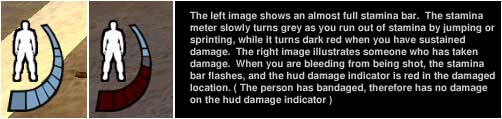
\includegraphics[scale=0.6]{Images/Hud_staminabar.jpg}
    \caption{\small Stamina bar in the HUD of Urban Terror (Source: \cite{urt}).}
    \label{fig:stamina}
  \end{figure}
  
  Two basic techniques will make your movements in the map more efficient: 
  \begin{enumerate}
  \item \emph{Wall jump}: while in the air after a jump or a fall, you can
    bounce on a wall (not necessary in front of you) by pressing jump (default:
    \texttt{SPACE}) when in contact with the wall. 
    You can even repeat this procedure up to 3 times to achieve more complex
    jump and reaching higher places.
  \item \emph{Strafe jump}: this name refers to a common technique in Quake III
    to reach a higher speed. It consists of changing side after each jump during
    a movement\footnote{Note that in Urban Terror and contrary to Quake III, you
      can't keep this procedure for long in a single run because of the stamina
      level.}.   
    For example:
    \begin{itemize}
    \item first sprint or run in a straight or curved line
    \item then jump and and keep turning left + hold left strafe
    \item jump and turn right + right strafe
    \item jump and turn left + left strafe etc. 
    \end{itemize}
    You will probably want to end this sequence by crouching (default key:
    \texttt{C}): it will make your character sliding to maintain the speed for a
    short while. You are able to affect the direction of the sliding using the
    directional key. Another important aspect is that while crouching in this
    way, you don't consume any more stamina and you're able to focus on a given
    point of interest.   
  \end{enumerate}
  For more details and techniques, please refer to the Jumping Guide available
  at \url{http://www.www0.org/cgi-bin/urtj}. 

\item[Exploit H.E. grenades tempo.] 
  Once unlocked, an HE grenade takes around 4 to 5 seconds to explode. You can
  play on this time to decide the best moment to throw it away:
  \begin{itemize}
  \item either immediately to protect a path or a place against incoming
    enemies: hopefully, the grenade will explode while they are reaching the
    place or prevent them from using it for a short while (Note that this also
    applied to HK69);  
  \item or after 3 to 4 seconds such that it explodes when reaching the floor
    such than the ennemy (typically hiden in a corner) won't have time to react
    and move to a safer place.   
  \end{itemize}
  Note that it is possible to unlock a grenade and switch to another weapon to
  cancel the unlocking for further use. This might be useful to avoid team kill
  and a more effective use of them even if I personally consider this as a bug.    
\item[Exploit smoke grenades.] They can cover your movements and be particularly
  effective when used in combination with tactical goggles: you will be able to
  locate incoming enemies and shoot with first strike.    
\end{description}


%----------------------------------
\subsection{Advanced configuration}
\label{sec:client:config}

Apart from the basic key bindings you can operate from the menu \texttt{SETUP}
$\rightarrow$ \texttt{CONTROLS} inside the game, the most useful aspect of UrT
is the capacity to fully customize the commands and the bindings use throughout
the game to reflect your own style of playing.  This is for instance very useful
for the radio commands.  

All the configuration resided in the configuration file \texttt{q3config.cfg},
located in the \texttt{q3ut4/} directory of your installed game, typically:
\begin{itemize}
\item[\windows]  \verb!C:\Program Files\UrbanTerror\q3ut4\!
\item[\linux]    \verb!~/.q3a/q3ut4/! (make sure to show hidden
  directories to find it)
\item [\macosx]  \verb!~/Library/Application Support/Quake3/q3ut4/!
\end{itemize}

\noindent My own configuration file is available at the following url:
\begin{center}
  \url{http://varrette.gforge.uni.lu/q3ut4/q3config.cfg}
\end{center}

\noindent The syntax of this file is inherited from Quake III Arena. I
will only insist on the \emph{binding} procedure. The general use of this
command is: 
\[ bind\  [key]\ "[command]" \]
You may configure multiple commands with a single key: just separate each
commands with a semicolon (;) so that UrT recognizes where each command starts
and stops. 
Note that you can color the text printed in the console using the escape
sequence \verb!^n! where \texttt{n} is a number between 1 and 8 according to the
following associations: 
\begin{center}
  \begin{tabular}[h]{clcl}
    1 & Red    & 2 & Green \\
    3 & Yellow & 4 & Blue  \\
    5 & Purple & 6 & Cyan  \\
    7 & White (Default) & 8 & Black 
  \end{tabular}
\end{center}
Example: "\verb!This text is ^1RED^7 and this one ^8BLACK!"

I will detail in this document the binding of 2 basic commands:
\texttt{ut\_radio} (\S\ref{sub:radio}) and \texttt{ut\_weaptoggle}
(\S\ref{sub:weapons}).  

%.....................................
\subsubsection{Radio command binding}
\label{sub:radio}


The \texttt{ut\_radio} command corresponds to
radio messages (use \texttt{U} to access the radio interface during the game -
see Figure~\ref{fig:radio}) yet it is important to bind the most useful radio
messages on a single key, especially if you want to display a colored message in
the console which is particularly pertinent for bomb site. 
Indeed, while the radio messages refer to them as A and B, they
correspond in practice to bomb site red and black so a colored message will help
your partner to identify more clearly the location you're speaking about.  
      
\begin{figure}[ht]
  \centering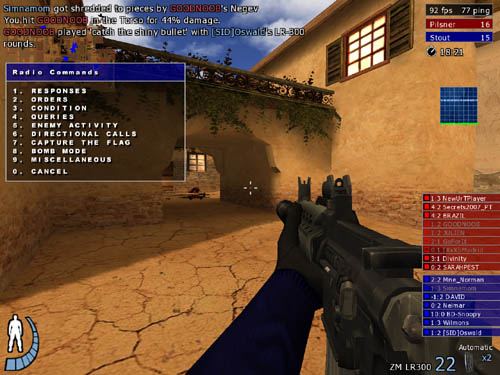
\includegraphics[scale=0.4]{Images/Ui_radiointerface.jpg}
  \caption{\small Radio interface during the game (first level) (Source: \cite{urt}).}
  \label{fig:radio}
\end{figure}

The table~\ref{tab:radio} summarizes the most important messages that justify
(for me) a binding and (eventually), a more pertinent message displayed on the
console. Several variables can be used in such messages, of greater importance stands: 
\begin{itemize}\setitemsep
\item \texttt{\$location}:  current position in the map;
\item \texttt{\$crosshair}: position in the map pointed by your crosshair;
\item \texttt{\$health}:    current health status.
\end{itemize}

Those preliminary comments being done, here is how to use the
table~\ref{tab:radio}. 
For each message, select a key to bind (let's say for instance \texttt{h} to the
radio message asking for a medic) then put the following line in your
\texttt{q3config.cfg}:
\begin{lstlisting}[style=filecontent]
bind h "ut_radio 3 3 I need a medic [^1status: $health^7] @ $location"
\end{lstlisting}
Eventually, if you don't want to overwrite the default message, simply use:
\begin{lstlisting}[style=filecontent]
bind h "ut_radio 3 3"
\end{lstlisting}


%\newcommand{\radio}[1]{\texttt{ut\_radio #1}}
\newcommand{\radio}[1]{\texttt{#1}}

\begin{table}[ht]
  \centering\small
  \begin{tabular}[h]{|c||c|l|}
    \hline
    \textbf{Type} & 
    \textbf{Menu} & \textbf{Proposed Message} \\ 
    \hline\hline
    \multirow{2}{*}{\textbf{Order}} 
                      & \radio{2 5} & \verb!Cover me @ $location! \\ 
                      & \radio{2 6} & \verb!Requesting backup @ $location!\\\hline
    \multirow{4}{*}{\textbf{Questions}}  
                       & \radio{3 2}  & \verb!Awaiting orders! \\ 
                       & \radio{3 3}  & \verb!I need a medic [^1status: $health^7] @ $location!\\
                       & \radio{4 2}  & \verb!Objective status?! \\
                       & \radio{4 4}  & \verb!Where's the enemy?! \\\hline
     \multirow{4}{*}{\textbf{Response}} 
                       & \radio{1 1} & \verb!Affirmative! \\ 
                       & \radio{1 2} & \verb!Negative! \\
                       & \radio{9 4} & \verb!Sorry about that! \\
                       & \radio{9 9} & \verb!Thanks! \\\hline
    \textbf{Activity}     & \radio{5 1} & \verb!Enemy spotted!\\\hline
    \multirow{6}{*}{\textbf{Bomb mode}}
                       & \radio{8 1} & \verb!Heading to bombsite ^1RED!\\
                       & \radio{8 2} & \verb!Heading to bombsite ^8BLACK!\\
                       & \radio{8 3} & \verb!Enemy at bombsite ^1RED!\\
                       & \radio{8 4} & \verb!Enemy at bombsite ^8BLACK!\\
                       & \radio{8 5} & \verb!I have the bomb @ $location!\\
                       & \radio{8 6} & \verb!The bomb is loose!!\\\hline
 
  \end{tabular}
  \caption{Most useful radio message in Urban Terror}
  \label{tab:radio}
\end{table}

You can find the full list of the radio messages in the manual of
UrT~\cite{urt}. 

%.....................................
\subsubsection{Weapon switch binding}
\label{sub:weapon}

By default, the keys 1 to 6 are assigned for the weapons from the knives to the
bomb. It appeared difficult for me to switch quickly with such a configuration
to the sidearm or the knife. That's where the \texttt{ur\_weaptoggle} command is
your friend. 
The format of this command is the following (replace \texttt{x} with the key to assign) : 
\begin{verbatim}
bind x "ut_weaptoggle [argument]"
bind x "ut_weaptoggle [argument] [argument]"
\end{verbatim}
where \texttt{argument} can be one of the following: \texttt{primary},
\texttt{secondary}, \texttt{sidearm}, \texttt{grenade}, \texttt{bomb} or
\texttt{knife}. 

The two argument version permits with the same key to switch from one class of
weapon to another.
For instance, I personally use the following configuration to easily switch from
the primary weapon to the sidearm (useful when in a battle where the magazine
becomes empty) or the knife (for a corporal combat): 
\begin{lstlisting}[style=filecontent]
bind f "ut_weaptoggle sidearm primary"
bind q "ut_weaptoggle knife primary"
\end{lstlisting}

%.......................................................
\subsubsection{Additional sources to tweak your configuration}

I just gave some basic elements of customization. 
You can go further using the following web site: 
\begin{itemize}\setitemsep
\item \url{http://q3ut3.free.fr/gear/} (UrbanTerror Gear script Generator)
  permits the binding of a single key to cycle between several configurations of
  weapons/equipment which can be useful at the beginning of a new map (for
  instance to quickly move from a sniper mod with SR8 to AK).
\item \url{http://ucguides.savagehelp.com/} provides a guide for Quake III where
  some information can be reuse for Urban Terror.
\end{itemize}

%----------------------
\subsection{New maps}

The best way to install new maps is to auto-download them from the server you
are playing. So normally, you have nothing to do (assuming the server is
configured correctly through the \texttt{sv\_dlURL} directive -- see
\S\ref{sec:server:install}).

Yet, you may want to install manually new maps. 
Apart from the basic maps, you can find community created levels on the
following website (ordered by personal preferences):
\begin{itemize}\setitemsep
\item \url{http://www.snipersgaulois.com/downloads.php}
\item \url{http://sex-e.clanservers.com/Downloads/c=1.html}
\item \url{http://urt.unfoog.de/q3ut4/}
\end{itemize}

Just put them into your \texttt{q3ut4/} directory.

Those sites propose in general a huge number of maps, some buggy and/or
unfinished. If you're only interested in pre-tested maps, you can take a look at
my own repository available at: \url{http://varrette.gforge.uni.lu/q3ut4/}




%~~~~~~~~~~~~~~~~~~~~~~~~~~~~~~~~~~~~~~~~~~~~~~~~~~~~~~~~~~~~~~~~
% eof
%
% Local Variables:
% fill-column: 80
% mode: latex
% mode: flyspell
% mode: auto-fill
% End:



%========================================================
\section{Linux server installation and configuration}
\label{sec:urt_server}
%=======================================================================
% File         : _server.tex
% Title        : 
% Author(s)    : Sebastien VARRETTE <Sebastien.Varrette@uni.lu>
% Creation     : 06 Jul 2009
% Time-stamp:    <2009-07-15 14:23:18 svarrette>
% $Id: _server.tex 447 2009-07-15 13:36:11Z svarrette $
% 
%   Copyright (c) 2009 Sebastien Varrette. 
%
% Licence: Creative Commons Attribution-Noncommercial-Share Alike 2.0 France
%
% You are free:
%   - to Share:  to copy, distribute and transmit the work
%   - to Remix: to adapt the work
%
% Under the following conditions:
%   - Attribution : You must attribute the work in the manner specified by the
%                   author or licensor (but  not in any way that suggests that
%                   they endorse you or your use of the work).  
%   - Noncommercial:  You may not use this work for commercial purposes.
%   - Share Alike: If you alter, transform, or build upon this work, you may
%                  distribute the resulting work only under the same or similar
%                  license to this one. 
%
% With the understanding that:
%   - Waiver: Any of the above conditions can be waived if you get permission from
%             the copyright holder. 
%   - Other Rights: In no way are any of the following rights affected by the
%                   license:  
%                    * Your fair dealing or fair use rights;
%                    * Apart from the remix rights granted under this license,
%                      the author's moral rights; 
%                     * Rights other persons may have either in the work itself
%                       or in how the work is used, such as publicity or privacy
%                       rights. 
%   - Notice:  For any reuse or distribution, you must make clear to others the
%              license terms of this work. The best way to do this is with a
%              link to this web page. 
%=======================================================================

%------------------------------
\subsection{Basic installation}
\label{sec:server:install}

This section describes the installation of a server under a Linux Debian
machine. 
First proceed to the Linux installation as stated in \S\ref{sec:urt_client}. 
Then create a dedicated user (\texttt{urbanterror}) for running the server,
attached to the group \texttt{urt}: 
\begin{lstlisting}[style=command]
[root@host]# adduser --system --ingroup urt urbanterror
\end{lstlisting}
The next step is to make this user owning the files coming with Urban Terror,
and creating the directory storing the logs and the pid files: 
\begin{lstlisting}[style=command]
[root@host]# chown -R urbanterror:urt /usr/local/games/urbanterror
[root@host]# mkdir /var/log/urbanterror /var/run/urbanterror
[root@host]# chown urbanterror:urt /var/log/urbanterror /var/run/urbanterror
[root@host]# ln -s ~urbanterror/.q3a/q3ut4/urt.log  /var/log/urbanterror/urt.log
\end{lstlisting}

As the server will be launched under the rights of the \texttt{urbanterror}
user, the log files of the server will be located  in
\verb!~urbanterror/.q3a/q3ut4/urt.log!. 
Le last instruction creates a symbolic link for the future log file of the
server in a more convenient place. 

\noindent You now have to decide about which server executable you want to use (either 32
bits \texttt{ioUrTded.i386} or 64 bits \texttt{ioUrTded.x86\_64}), make it
executable and create the link to it. 
It follows that for running a 32 bits executable, you will typically run the
following commands: 
\begin{lstlisting}[style=command]
[root@host]# cd /usr/local/games/urbanterror
[root@host]# chmod +x  ioUrTded.i386
[root@host]# ln -s ioUrTded.i386 urbanterror.server  
\end{lstlisting}

\noindent If you followed exactly this tutorial, the configuration file of the server
resides in  
\texttt{/usr/local/games/urbanterror/q3ut4/server.cfg}. 
It is nicely commented so you shouldn't have trouble to adapt it to reflect your
own configuration. 
Yet here are the variables you should pay attention: 
\begin{lstlisting}[style=urtcfg]
sets " Admin" "yourname" 
sets " Email" "xxx@xxx.xxx"

set sv_hostname "your server name, by xxx" 
set g_motd "Your stats on xxx" //Your message of the day here, 
set sv_joinmessage "Welcome to Urban Terror 4.1"  //Your joinmessage here

sets sv_dlURL "urt.unfoog.de" // use this server instead of teh default one

set g_gametype "8" // default to bomb mode ;)

set rconpassword "xxx" //Password to control the server remotely using rcon.

set sv_master2 ""  // leave those empty to prevent notifications of master 
set sv_master3 ""  // servers about your server. 
set sv_master4 ""

set g_log "urt.log" // name of the log file
//*** B3 Specific settings ***
set g_logSync "3"     //XLR: Unbuffered/direct logging for B3
set sv_zombietime "6" //XLR: Larger zombietime to reduce slot/client mixups for B3
set g_loghits "1" //XLR: headshotcounter and XLRstats bodypart information for B3
\end{lstlisting}

The \texttt{server.cfg} I'm currently using for my own server is proposed in
appendix~\ref{anx:server.cfg}, page~\pageref{anx:server.cfg}\\

Now you should be able to start the server. On Debian, you should be addicted to
have a script for startup in the directory \texttt{/etc/init.d/}.
It appeared difficult to find one so I made one proposed in
appendix~\ref{anx:init.d:urbanterror} page~\pageref{anx:init.d:urbanterror}. 
Put this script in the folder \texttt{/etc/init.d/}, make it
executable (\texttt{chmod +x /etc/init.d/urbanterror}). You can now start the
server by issuing the command: 
\begin{lstlisting}[style=command]
[root@host]# /etc/init.d/urbanterror start
\end{lstlisting}

Now your server is running and should be seen from the client software of your
network. Check that you can play on the server, vote to cycle, change map etc. 
Once ensured that the server is working fine, you can continue to
section~\ref{sec:b3} to configure Big Brother Bot and make your server even more  
powerful. 

%--------------------------------------------------------------------------
\subsection{Installing new maps and adapting the \texttt{mapcycle.txt} file}
\label{sec:server:new:map}

To install a new map on your server, you have several steps to do: 
\begin{enumerate}
\item copy the map file (typically \texttt{ut4\_mapname.pk3}) into the folder\\
  \texttt{/usr/local/games/urbanterror/q3ut4/}; 
\item ensure the map file is available for auto-download on the server you
  configured with the directive \texttt{sv\_dlURL} in \texttt{server.cfg} (see
  \S\ref{sec:server:install});
\item adapt your \texttt{mapcycle.txt} file to include your new map in the map
  list (see my script \texttt{createmapcycles.sh} below);
\item change the \texttt{map} directive at the end of your \texttt{server.cfg}
  to  \texttt{ut4\_mapname} (remove the extension) such that n restart, the new
  map will be proposed directly;
\item restart the server by issuing the following command: 
  \begin{lstlisting}[style=command]
    [root@host]# /etc/init.d/urbanterror restart
  \end{lstlisting}
\end{enumerate}

\noindent To automatically handle new maps and randomizing the maps in the
\texttt{mapcycle.txt} file, I wrote two scripts: 
\begin{itemize}
\item \texttt{createmapcycles.sh}, to be put together with the file
  \texttt{mapcycle.txt.orig} in the directory
  \texttt{/usr/local/urbanterror/q3ut4/} (both proposed in
  appendix~\ref{anx:mapcycle:all} page~\pageref{anx:mapcycle:all}). \\
  This script is responsible for creating a file named \texttt{mapcycle.txt.all}
  listing the default maps (taken from \texttt{mapcycle.txt.orig}) and all newly
  added maps (detecting by a simple \texttt{ls} command on the files in the
  directory with format \texttt{ut4\_*}).
\item \texttt{randomize\_mapcycle.pl} that randomizes the entries of a file
  listing the maps to be put in the final \texttt{mapcycle.txt}. 
  This Perl script should be placed in the directory
  \texttt{/usr/local/urbanterror/q3ut4/}.  
\end{itemize}
 
The first script (\texttt{createmapcycles.sh}) is typically launched once for
each newly installed map, \emph{i.e.} between the steps 4 and 5 described at the
beginning of this section. 

On the contrary, the second script is typically launched every time the server
is started. If you want to activate this feature, simply uncomment the line
defining the variable \texttt{MAPCYCLE\_RANDOMIZE\_SCRIPT} in the startup script
proposed in appendix~\ref{anx:init.d:urbanterror}.


%~~~~~~~~~~~~~~~~~~~~~~~~~~~~~~~~~~~~~~~~~~~~~~~~~~~~~~~~~~~~~~~~
% eof
%
% Local Variables:
% fill-column: 80
% mode: latex
% mode: flyspell
% mode: auto-fill
% End:


%============================================================
\section{Big Brother Bot installation and configuration}
\label{sec:b3}
%=======================================================================
% File         : _b3.tex
% Title        : 
% Author(s)    : Sebastien VARRETTE <Sebastien.Varrette@uni.lu>
% Creation     : 06 Jul 2009
% Time-stamp:    <Thu 2012-07-26 11:35 svarrette>
%   
%   Copyright (c) 2009 Sebastien Varrette. 
%
% Licence: Creative Commons Attribution-Noncommercial-Share Alike 2.0 France
%
% You are free:
%   - to Share:  to copy, distribute and transmit the work
%   - to Remix: to adapt the work
%
% Under the following conditions:
%   - Attribution : You must attribute the work in the manner specified by the
%                   author or licensor (but  not in any way that suggests that
%                   they endorse you or your use of the work).  
%   - Noncommercial:  You may not use this work for commercial purposes.
%   - Share Alike: If you alter, transform, or build upon this work, you may
%                  distribute the resulting work only under the same or similar
%                  license to this one. 
%
% With the understanding that:
%   - Waiver: Any of the above conditions can be waived if you get permission from
%             the copyright holder. 
%   - Other Rights: In no way are any of the following rights affected by the
%                   license:  
%                    * Your fair dealing or fair use rights;
%                    * Apart from the remix rights granted under this license,
%                      the author's moral rights; 
%                     * Rights other persons may have either in the work itself
%                       or in how the work is used, such as publicity or privacy
%                       rights. 
%   - Notice:  For any reuse or distribution, you must make clear to others the
%              license terms of this work. The best way to do this is with a
%              link to this web page. 
%=======================================================================

Big Brother Bot B3~\cite{b3} is a complete and total server administration
package for online games. 
B3 is based on the analysis of the log files populated by a running server. 
It means that as soon as B3 is able to parse and interpret the logs of a given
game, this game is supported. This is the case for Urban Terror. 
The main interest of B3 resides in the fact that the administrations tasks are
handled by plugins written by the community yet with a common interface and
installation procedure. This makes B3 very flexible and easy to use. 

I detail here the configuration of B3 on your Linux server, assuming you
followed the instructions proposed in the previous section.

Note that your main source of information should be the official guidelines
provided at the following url:\\ 
\url{http://wiki.github.com/BigBrotherBot/big-brother-bot/installation}

If you experience any problem, don't hesitate to use B3 forum available at 
\url{http://www.bigbrotherbot.com/forums} 

%--------------------------
\subsection{Prerequisites}
\label{sec:b3:prerequisite}

Several components are required before installing B3 in itself: 
\begin{itemize}
\item A MySQL server and therefore PhPMyAdmin and a Web server (the later being
  mandatory for \texttt{xlrstats}).
  Under Debian, just run: 
  \begin{lstlisting}[style=command]
[root@host]# apt-get install apache2 mysql-server phpmyadmin
[root@host]# ln -s /usr/share/phpmyadmin/ /var/www/phpmyadmin
  \end{lstlisting}
  For the configuration, see below. 
\item some Python stuff (\url{http://www.python.org}), more particularly: 
  Python 2.3+, Elementtree, Python-MySQL and Python Setuptools. Under Debian,
  simply run: 
  \begin{lstlisting}[style=command]
[root@host]# apt-get install python2.5 python-elementtree \ 
             python-mysqldb python-setuptools
  \end{lstlisting}
\end{itemize}

%.....................................
\subsubsection{Web server configuration}
\label{sub:b3:apache}

As you plan to use phpMyAdmin, it is mandatory to activate SSL support for the
Web server, which means you will have to create a certificate for it.
This requires \texttt{OpenSSL} so install it: 
  \begin{lstlisting}[style=command]
[root@host]# apt-get install openssl
  \end{lstlisting}

Then get the fully qualified host name of the server (run \texttt{hostname -f}
typically), or use the future url of your server. 
In the sequel, I'll assume the server to be reached by the name
\texttt{myurtserver.domain.com}. 
To create the certificates (valid for 1414 days), run:  
  \begin{lstlisting}[style=command]
[root@host]# cd /etc/apache2/
[root@host]# mkdir ssl.key ssl.crt ssl.crl
[root@host]# chmod 700 ssl.key
[root@host]# openssl req -new -x509 -days 1414 -nodes \ 
   -keyout /etc/apache2/ssl.key/server.key -out /etc/apache2/ssl.crt/server.crt \ 
   -subj '/O=COM/OU=DOMAIN/CN=myurtserver.domain.com'
  \end{lstlisting}
I don't know how familiar you are with SSL certification, yet you should adapt
the subject of the certificate (precised with \texttt{-subj}) to reflect your
own structure (for the \texttt{O}rganization name (\texttt{COM} here) and your
\texttt{O}rganization \texttt{U}nit name (\texttt{DOMAIN} here). The critical
point is to place your server fully qualified name as \texttt{C}ommon
\texttt{N}ame.
For more information, read the \texttt{README} file coming with apache2: 
\begin{lstlisting}[style=command]
  [root@host]# zless /usr/share/doc/apache2.2-common/README.Debian.gz
\end{lstlisting}

This creates a self-signed certificate \texttt{/etc/apache2/ssl.crt/server.crt}
and the associated private key \texttt{/etc/apache2/ssl.crt/server.key}. 
Now you should notify the SSL module of Apache about the location of those
certificates. 
Edit \texttt{/etc/apache2/mods-available/ssl.conf} and add/update the
properties as follows: 
\begin{lstlisting}[style=apachecfg]
<IfModule mod_ssl.c>
  ...
  # The certificates of the server to use
  SSLCertificateFile      /etc/apache2/ssl.crt/server.crt
  SSLCertificateKeyFile   /etc/apache2/ssl.key/server.key
  ...
</IfModule>
\end{lstlisting}
Now comment the \texttt{NameVirtualHost} directive in \texttt{/etc/apache2/ports.conf}.
Then activate the SSL module (together with the rewrite one): 
\begin{lstlisting}[style=command]
[root@host]#  a2enmod ssl
[root@host]#  a2enmod rewrite
\end{lstlisting}

\noindent You should now update the file configuring the web server by editing
the file \texttt{/etc/apache2/site-available/default} as follows:  
\lstinputlisting[caption=The \texttt{/etc/apache2/site-available/default}
configuration file for your Apache server,style=apachecfg,basicstyle=\scriptsize]{../config_files/apache2/site-default}

\noindent Now start the web server by running:
\begin{lstlisting}[style=command]
[root@host]# apache2ctl restart
\end{lstlisting}
(You can also use "\texttt{/etc/init.d/apache2 restart}"). Check that the server
works by opening a browser in the url \url{http://myurtserver.domain.com}. 
You should be automatically redirect to the url
\url{https://myurtserver.domain.com}.  

%.....................................
\subsubsection{MySQL configuration}
\label{sub:b3:mysql}

Assuming the MySQL server to be running (\texttt{/etc/init.d/mysql restart}
eventually), you should be able also to use PHPMyAdmin by accessing to the url 
\url{https://myurtserver.domain.com/phpmyadmin/}.
Note that the server is configured the authorize the access to this interface
only for the machine with the IP address \texttt{your.ip.adress.here} according
to configuration of the Apache server (see \S\ref{sub:b3:apache}). 
In case of trouble, your very first reflex (as always) is to check the problem
in the logs. To check them online, run in a separate terminal (CTRL-C to quit): 
\begin{lstlisting}[style=command]
[root@host]# tail -f /var/log/apache2/error.log
\end{lstlisting}

In all case, once you're able to interact with the MySQL server, your very first
task is to setup a root password for it (blank by default). 
Prefer using PHPMyAdmin for that (go to the Privilege section) or run the
following command (just ensure you flush by after the history of the commands to
avoid password retrieval -- this is not perfect but a minimum security measure):
\begin{lstlisting}[style=command]
[root@host]# mysqladmin -u root password "your_password_here"
[root@host]# history -c
\end{lstlisting}

Using PHPMyAdmin, create a MySQL user \texttt{b3} (generate a random password
for him and keep it in a safe place such as an encrypted file) with full right
on a database named \texttt{b3}. 
Create also a MySQL user \texttt{b3\_ro} with read-only access to the database
\texttt{b3} (\emph{i.e.} with privileges limited to the \texttt{SELECT}
command). Again, generate a random password for him and keep it in a safe
place. 
In the sequel, I'll assume those users to be configured as follows: 
\begin{itemize}\setitemsep
\item MySQL user \texttt{b3}: password \texttt{\_\_b3\_password\_\_};
\item MySQL user \texttt{b3\_ro}: password \texttt{\_\_b3\_ro\_password\_\_}.
\end{itemize}
 
%--------------------------
\subsection{B3 installation}
\label{sec:b3:install}

You are now ready to install B3 (When writing this tutorial, the latest release
of B3 was the version 1.1.4b). 
Simply run:
\begin{lstlisting}[style=command]
[root@host]# easy_install -U b3
\end{lstlisting}
\emph{Note:} this will install b3 in the following directory: \\
\texttt{/usr/lib/python2.5/site-packages/b3-1.1.4b-py2.5.egg/b3} \\
In the sequel and to make things simpler (and shorter), I will refer to this
directory as \begginstall.

%...................................
\subsubsection{Preparing the database}
\label{sec:b3:dbsetup}

Retrieve the file \begginstall\texttt{/doc/b3.sql} from the server (typically
using \texttt{scp}). 
Then, use PHPMyAdmin to connect to the database \texttt{b3} (created during the process
described in \S\ref{sub:b3:mysql}) as user \texttt{b3}.
Select the menu \texttt{Import}, then choose the previously retrieved file,
\texttt{b3.sql} and finally click on \texttt{Go}. 
This should populate the database \texttt{b3} with the tables required by Big
Brother Bot.  

%...........................
\subsubsection{B3 Configuration}
\label{sec:b3:config}

Create the directory structure for hosting the B3 configuration as follows: 
\begin{lstlisting}[style=command]
[root@host]# mkdir ~urbanterror/b3
[root@host]# cd ~urbanterror/b3
[root@host]# mkdir -p conf extplugins/conf init.d plugins_toinstall
[root@host]# cp $B3_EGG_INSTALLDIR/conf/* ~urbanterror/b3/conf/
[root@host]# ln -s /var/log/urbanterror/b3.log b3.log
[root@host]# chown -R urbanterror:urt ~urbanterror/b3
\end{lstlisting}%$

The main configuration file for B3 is named \texttt{b3.xml} and is located in
the directory \texttt{/home/urbanterror/b3/conf/}. 
Edit and adapt it as the one proposed in appendix~\ref{anx:b3:b3.xml}
page~\pageref{anx:b3:b3.xml}. 
In particular, it is very important to disable PunkBuster otherwise you will get
the error message "\emph{[pm] Please try your command after you have been
  authenticated}" when playing on the server and trying to register.

The configuration proposed in appendix~\ref{anx:b3:b3.xml} activate a single
plugin called \texttt{admin}. 
This is for a first check and we will see later how to add and activate new
plugins. 

The only step missing for the installation is a startup script to manage B3 
\texttt{/etc/init.d/bigbrotherbot}.  
Mine is proposed in appendix~\ref{anx:init.d:b3} page~\pageref{anx:init.d:b3}.  
Assuming your UrT server is running (\emph{i.e.} the log files are populated),
you should be able to launch b3 as follows: 
\begin{lstlisting}[style=command]
[root@host]# /etc/init.d/bigbrotherbot start
\end{lstlisting}

To check this is working, connect to the server and once in the game, type as a
message \verb/!register/. This will register yourself in B3 (assuming your
player name is \texttt{Toto}, you should receive as an answer in the console the
fact that \texttt{Toto} has been put in the \texttt{User} group. 
In all case, detect the anomalies by monitoring the log files of b3 and running
in a separate terminal:
\begin{lstlisting}[style=command]
[root@host]# tail -f /var/log/urbanterror/b3.log
\end{lstlisting}

\noindent 
You shall now familiarize yourself with the commands available under B3 with the
plugin \texttt{admin}. 
For this, you shall refer to the official manual available at: 
\texttt{http://wiki.github.com/BigBrotherBot/big-brother-bot/manual-commands}\\

You will notice that each command comes with a level to authorize or not the
access to the command. 
To make yourself admin of B3 (\emph{i.e.} able to launch all commands), the best
is to update the table \texttt{clients} in the \texttt{b3} database. 
Locate the entry with your player name (field \texttt{name}). 
The value associated to your name in the \texttt{group\_bits} fields should be
1. This translate the fact that you have been put in the User group. 
Change this value to 128 to make you an admin of B3. 
%
You might want to delegate some administration tasks to other players. 
For this, make their \texttt{group\_bits} to 20 typically. 

%--------------------------------------------
\subsection{Configuring the default plugins}
\label{sec:b3:plugins}

B3 comes with a few plugins more or less relevant for Urban Terror summarized in
Table~\ref{tab:b3:plugins}. 
\begin{table}[ht]
  \centering\small
  \begin{tabular}{|c|p{0.8\textwidth}|}
    \hline
    \texttt{admin} & Provides the majority of B3 functionality such as kicking,
    banning, user management, and warnings\\
    \texttt{adv} & Advertise messages periodically\\
    \texttt{censor} & Warn users when using banned words\\
    \texttt{stats} & Simple transient stats that track stats while the users
    is connected\\ 
    \texttt{pingwatch} & Warn users for high/low pings and kick when the ping
    goes to high\\ 
    \texttt{spamcontrol} & Warn users for saying too many messages in a short
    period of time\\ 
    \texttt{status} &  Dumps an XML file to the server periodically with B3 and
    user information to be used on your website to display game status \\
    \texttt{tk} & Monitors team damage and team kills\\ 
    \texttt{welcome} &Welcome messages for new and returning users\\\hline 
  \end{tabular}
  \caption{Default plugins proposed with Big Brother Bot}
  \label{tab:b3:plugins}
\end{table}

\noindent Until now, B3 is configured with the \texttt{admin} plugin enabled. 
Before going further, a few elements should be known about the plugins for B3:
\begin{itemize}
\item A given plugin \texttt{toto} is written in Python in a file named
  \texttt{toto.py}. This file is located in \begginstall\texttt{/plugins/} (this
  holds for the default plugins).
  On startup, B3 eventually compile this plugin to generate a new file
  \texttt{toto.pyc} for a more efficient execution. 
  Therefore if for any reason you decide to modify the source file of a plugin,
  remember to delete the compiled file before restarting B3. Otherwise your
  modification won't be taken into account.
  You may claim you will nether modify plugins sources files, yet it may happens
  if you want to change the position in the screen where a given message is
  displayed. You can alter this location as follows:
  \begin{itemize}
  \item Upper left (server announce area): 
    \texttt{self.console.write('blabla')} or \texttt{self.console.broadcast('blabla')}
  \item Lower left (chat area): \texttt{self.console.say('blabla')}
  \item Center screen (Big text): \texttt{self.console.write('bigtext blabla')}
  \end{itemize}



\item A given  plugin \texttt{toto} comes with a configuration file
  \texttt{plugins\_toto.xml} that respects the following format: 
  \begin{lstlisting}[language=xml,numbers=none,]
<configuration plugin="toto">
  ...
</configuration>    
  \end{lstlisting}
  This configuration files is located by default in \begginstall\texttt{/conf/}
  yet remember that I preferred to put the default configurations files in    
  \texttt{/home/urbanterror/b3/conf/}.
  Actually, the exact location of plugins configuration files is specified by
  the \texttt{config} attribute of the \texttt{plugin} anchor used in the
  configuration file \texttt{b3.xml}.
\item External plugins are handled in a separate directory, either in the
  default location \begginstall\texttt{/extplugins/} or, in the hierarchy
  proposed in this document, in \texttt{/home/urbanterror/b3/extplugins/}.\\
  This directory will contain the Python sources files of the plugins together
  with a sub-directory \texttt{conf/} which host the plugins configuration
  files.
\item Activating a plugin is done through the configuation file \texttt{b3.xml} in
  the \texttt{plugins} section.  
  Each plugin is characterized by a name, a unique priority value (within the
  list of your plugins) and a path to
  the configuration file as follows: 
  \begin{lstlisting}[style=apachecfg]
<plugins>
   <plugin name="plugin_name" priority="n"  config="/path/to/plugin_conf.xml"/>
</plugins>
  \end{lstlisting}
  The name provided should correspond to the basename of the Python source file
  (without the extension \texttt{.py}).  
  B3 will search for such a file in the default installation directory
  (\emph{i.e.} \begginstall\texttt{/}), then in the default external plugin
  directory (\emph{i.e.}  \begginstall\texttt{/extplugins/}) and finally in a
  user-defined external directory specified in a \texttt{settings} section of
  \texttt{b3.xml}. \\
  For instance, in the configuration files proposed in
  appendix~\ref{anx:b3:b3.xml}, we setup this external directory to
  \texttt{/home/urbanterror/b3/extplugins} as follows:
  \begin{lstlisting}[style=apachecfg]
<settings name="plugins">
   <set name="external_dir">/home/urbanterror/b3/extplugins</set>
</settings>
  \end{lstlisting}
  Note that when specifying the path to the plugin configuration file, you can
  use the sequence \texttt{@b3/} to refer to \begginstall\texttt{/}. 
\end{itemize}

\noindent You can now activate one of the default plugins summarized in the
table~\ref{tab:b3:plugins}.  For instance to activate the plugin
\texttt{welcome}: 
\begin{enumerate}\setitemsep
\item Examine \texttt{/home/urbanterror/b3/conf/plugin\_welcome.xml} to
  eventually adapt the configuration to suits your needs;
\item Select a priority value $n$ (3 in the sequel) and add a new
  \texttt{plugin} anchor in the \texttt{plugins} section of \texttt{b3.xml}:
  \begin{lstlisting}[style=apachecfg]
<plugins>
   ...
   <plugin name="welcome" priority="3" 
           config="/home/urbanterror/b3/conf/plugin_welcome.xml"/>
</plugins>
  \end{lstlisting}
\item Restart B3:
\begin{lstlisting}[style=command]
[root@host]# /etc/init.d/bigbrotherbot restart
\end{lstlisting}
\end{enumerate}

%--------------------------------------------------------------------------
\subsection{General procedure to install third party plugins}
\label{sec:b3:extplugins}

The flexibility of B3 permits the availability of various third party plugins. 
You will find them in the \texttt{Plugins/Releases} section of the Big Brother Bot forum
(indeed a very nice source of info for you): 
\begin{center}
  \url{http://www.bigbrotherbot.com/forums/index.php?board=17.0}
\end{center}

\noindent 
On this page, you should find a list of released plugins, each of them coming
with a short description, a download location and an install guide. 
You shall always refer to the install guide yet here is the general procedure to
install and configure a third plugin. 
To make this procedure concrete, I'll illustrate it on the \texttt{heashotsurt}
plugin (version \texttt{0.2.0}) which counts the number of headshot kills made
by the players: 
\begin{enumerate}
\item Download the plugin sources \texttt{heashotsurt-v0.2.0.zip} and unzip this
  file into the folder:\\
  \texttt{/home/urbanterror/b3/plugins\_toinstall/heashotsurt-v0.2.0}
\item Copy (or make a symbolic link of) the Python source file
  \texttt{heashotsurt.py} into the external plugin directory 
  \texttt{/home/urbanterror/b3/extplugins/}
\item Copy (or make a symbolic link of) the  configuration file
  \texttt{headshots.xml} into the  external plugin configuration directory\\ 
  \texttt{/home/urbanterror/b3/extplugins/conf/}
\item As for default plugins, select a unique priority value $n$ (14 for
  instance) and add a new \texttt{plugin} anchor in the \texttt{plugins} section
  of \texttt{b3.xml}:
  \begin{lstlisting}[style=apachecfg]
   <plugin name="headshotsurt" priority="14"  
           config="/home/urbanterror/b3/extplugins/conf/headshots.xml"/>
  \end{lstlisting}
\item Restart B3:
\begin{lstlisting}[style=command]
[root@host]# /etc/init.d/bigbrotherbot restart
\end{lstlisting}
\end{enumerate}

\noindent This procedure holds for most of the external plugins. 
I personally installed in this way the following plugins: 
\begin{itemize}\setitemsep
\item \texttt{PowerAdminUrt} (version \texttt{1.4.0b3})\\
  {\small \url{http://www.bigbrotherbot.com/forums/index.php?topic=426.0}}\\
  Remember to edit the file \texttt{extplugins/conf/poweradminurt.xml} and
  disable the \texttt{rotationmanager} by putting the value False as follows:
  \begin{lstlisting}[style=apachecfg]
<settings name="rotationmanager">
    <!-- enable the rotationmanager? -->
    <set name="rm_enable">False</set>
    ...
</settings> 
 \end{lstlisting}
\item \texttt{headshotsurt} (version \texttt{0.2.0}) \\ 
  {\small \url{http://www.bigbrotherbot.com/forums/index.php?topic=367.0}}
\item \texttt{topkiller} (version \texttt{1.0.4})\\
  {\small\url{http://www.bigbrotherbot.com/forums/index.php?topic=574.0}}
\item \texttt{Spree} (version \texttt{1.1})\\
  {\small\url{http://www.bigbrotherbot.com/forums/index.php?topic=864.0}}
\end{itemize}

I now dedicated a full section to one of the most interesting external plugin
which comes with B3: \texttt{xlrstats}

%--------------------------------------------------------------------------
\subsection{Installing XLRstats}
\label{sec:b3:xlrstats}

XLRstats (\url{http://www.xlrstats.com/}) is a statistics plugin for
BigBrotherBot (B3) and it stores all kill-events in the MySQL database used by
B3.
Stats are available in real time in the game using the \texttt{!xlrstats} command in
chat, but much more can be viewed in the XLRstats webfront (such as weapon
usage, ranks, medals etc.).
The sources of the plugin are part of B3 installation (we won't touch them). 
You still need to download the following elements (put them
into \verb!~urbanterror/b3/plugins_toinstall/!):
\begin{itemize}\setitemsep
\item The latest webfront \texttt{xlrstats-web-v2} (version 2.0.6), available on\\
 \url{http://github.com/xlr8or/xlrstats-web-v2/tree};
\item The image pack for UrT (\texttt{xlrstats-imagepack-urt}), to get from\\
  \url{http://xlr8or.snt.utwente.nl/forum/index.php?action=downloads}. 
\end{itemize}

\noindent 
You first need to create the extra tables in the \texttt{b3} database. 
The procedure is similar to the one explained in \S\ref{sec:b3:dbsetup}, this
time using the file present in the sub-directory 
\texttt{xlrstats-web-v2/xlrstats/sql/xlrstats.sql}

\noindent 
Once this is done, two B3 plugins should be installed: 
\begin{enumerate}
\item \texttt{status}, one of the default plugins (see \S\ref{sec:b3:plugins}). \\
  Just edit \texttt{/home/urbanterror/b3/conf/plugin\_status.xml} as follows:
  \begin{lstlisting}[style=apachecfg]    
<configuration plugin="status">
	<settings name="settings">
		<set name="interval">60</set>
		<set name="output_file">/var/www/status.xml</set>
	</settings>
</configuration>
  \end{lstlisting}
  This will configure the plugin to populate the file
  \texttt{/var/www/status.xml} for which the web server should have read
  access. In this purpose, run the following commands: 
  \begin{lstlisting}[style=command]
[root@host]# touch /var/www/status.xml
[root@host]# chown urbanterror:www-data /var/www/status.xml
[root@host]# chmod 644 /var/www/status.xml
  \end{lstlisting}
\item the \texttt{ctime} plugin that comes with XLRStats webfront in
  the zip file \texttt{b3-plugins/ctime.zip}. Once unpacked, 
  create the extra tables in the \texttt{b3} database using the
  \texttt{ctime.sql} file (re-use the procedure proposed in
  \S\ref{sec:b3:dbsetup}). 
  Then configure the plugin as explained in \S\ref{sec:b3:extplugins}.
\end{enumerate}

\noindent As always, the plugins are enabled in B3 as soon as you add them in the
\texttt{plugins} section of \texttt{b3.xml} (just adapt the priority values eventually): 
  \begin{lstlisting}[style=apachecfg]
<plugins>
   ...
   <plugin name="xlrstats" priority="2"  config="@b3/extplugins/conf/xlrstats.xml"/>
   ...
   <plugin name="status" priority="10"  
           config="/home/urbanterror/b3/conf/plugin_status.xml"/>
   <plugin name="ctime"  priority="11"
           config="/home/urbanterror/b3/extplugins/conf/plugin_ctime.xml"/>
   ...
</plugins>
  \end{lstlisting}

\noindent 
Restart B3 and ensure everything is working correctly (check the log file \\
\texttt{/var/log/urbanterror/b3.log} eventually). 
Now we can setup the webfront (take a look at \url{http://www.xlrstats.com/} for
the reference webfront documentation). 
First copy the files of the webfront into a more convenient place:
\begin{lstlisting}[style=command]
[root@host]# cd /home/urbanterror/b3/plugins_toinstall/xlrstats-web-v2/xlrstats
[root@host]# cp -r xlrstats /usr/share/
[root@host]# cd ../../
[root@host]# cp -r xlrstats-imagepack-urt/images/* /usr/share/xlrstats/images/
[root@host]# chown -R urbanterror:www-data /usr/share/
[root@host]# chmod -R g+r /usr/share/xlrstats
[root@host]# ln -s /usr/share/xlrstats/ /var/www/xlrstats
\end{lstlisting}

\noindent 
Then make the folders \texttt{dynamic} and \texttt{config} writable by the
webserver:
\begin{lstlisting}[style=command]
[root@host]# chmod 770 /var/www/xlrstats/dynamic
[root@host]# chmod 770 /var/www/xlrstats/config
\end{lstlisting}

\noindent 
Update \texttt{/etc/apache2/sites-available/default} to include
the \texttt{xlrstats} directory (typically to limit access to it to a few IP addresses):
\begin{lstlisting}[style=apachecfg]
<Directory /var/www/xlrstats/>
        Order Deny,Allow
        Deny from all
	Allow from 127.0.0.1
        Allow from toto.ip.address
	Allow from tata.ip.address	
</Directory>

<VirtualHost xx.yy.zz.tt:443>
        ...
        Alias /stats  /var/www/xlrstats
        ...
</VirtualHost>

\end{lstlisting}
Finally restart the web server: 
\begin{lstlisting}[style=command]
[root@host]# apache2ctl restart
\end{lstlisting}

\noindent 
Now go to the url \url{http://myurtserver.domain.com/stats/install/}
Select "\emph{Start Install}", then "\emph{Next}". 
In the "MySQL Connection Settings" panel, enter the following configuration (adapt the password): 
\begin{itemize}\setitemsep
\item Host name: \texttt{localhost}
\item MySQL Username : \texttt{b3\_ro}
\item MySQL Password: \texttt{\_\_b3\_ro\_password\_\_}
\item MySQL Database Name: \texttt{b3}
\end{itemize}
In the "Basic Game \& Server Settings", make sure you select the game Urban
Terror, enter the public IP of the server (\texttt{xx.yy.zz.tt:27960} -- see
\S\ref{sub:b3:apache}).  The B3 status url is
\url{http://myurtserver.domain.com/status.xml}

Once everything is done, a file \texttt{config/statsconfig.php} is created. 
Ensure this file has the permissions \texttt{750}. 
You should now go to the url\\
\url{http://myurtserver.domain.com/stats/config/install_award_idents.php} to
setup the medals etc. (actually, you should do it every time you experience a
trouble with awards). You can now delete the \texttt{install} directory and
enjoy XLRStats at \url{http://myurtserver.domain.com/stats/}. 


%~~~~~~~~~~~~~~~~~~~~~~~~~~~~~~~~~~~~~~~~~~~~~~~~~~~~~~~~~~~~~~~~
% eof
%
% Local Variables:
% fill-column: 80
% mode: latex
% mode: flyspell
% mode: auto-fill
% End:



\clearpage
\appendix

%====================
\section{Appendix}
\label{sec:anx}
%=======================================================================
% File         : _appendix.tex
% Title        : 
% Author(s)    : Sebastien VARRETTE <Sebastien.Varrette@uni.lu>
% Creation     : 06 Jul 2009
% Time-stamp:    <Thu 2012-06-28 00:27 svarrette>
%
% $Id$ 
% 
%   Copyright (c) 2009 Sebastien Varrette. 
%
% Licence: Creative Commons Attribution-Noncommercial-Share Alike 2.0 France
%
% You are free:
%   - to Share:  to copy, distribute and transmit the work
%   - to Remix: to adapt the work
%
% Under the following conditions:
%   - Attribution : You must attribute the work in the manner specified by the
%                   author or licensor (but  not in any way that suggests that
%                   they endorse you or your use of the work).  
%   - Noncommercial:  You may not use this work for commercial purposes.
%   - Share Alike: If you alter, transform, or build upon this work, you may
%                  distribute the resulting work only under the same or similar
%                  license to this one. 
%
% With the understanding that:
%   - Waiver: Any of the above conditions can be waived if you get permission from
%             the copyright holder. 
%   - Other Rights: In no way are any of the following rights affected by the
%                   license:  
%                    * Your fair dealing or fair use rights;
%                    * Apart from the remix rights granted under this license,
%                      the author's moral rights; 
%                     * Rights other persons may have either in the work itself
%                       or in how the work is used, such as publicity or privacy
%                       rights. 
%   - Notice:  For any reuse or distribution, you must make clear to others the
%              license terms of this work. The best way to do this is with a
%              link to this web page. 
%=======================================================================

\textbf{Important Note}: the scripts provided in this appendix are available for
download at the following url: 
\begin{center}
  \url{http://varrette.gforge.uni.lu/q3ut4/../config_files/}
\end{center}

%-------------------------------------------
\subsection{My personal \texttt{server.cfg}}
\label{anx:server.cfg}

\lstinputlisting[caption=The \texttt{/usr/local/urbanterror/q3ut4/server.cfg} configuration file,style=urtcfg,basicstyle=\scriptsize]{../config_files/q3ut4/server.cfg}

%----------------------------------------
\subsection{\texttt{/etc/init.d/urbanterror}}
\label{anx:init.d:urbanterror}

Remember to make this script executable (\texttt{chmod +x}) once copied in the
directory \texttt{/etc/init.d/}.

\lstinputlisting[caption=The startup script \texttt{/etc/init.d/urbanterror},style=urtcfg,basicstyle=\scriptsize]{../config_files/init.d/urbanterror}


%------------------------------------------------------------------
\subsection{Automatic generation of the file \texttt{mapcycle.txt.all}
  containing all maps available on the server}
\label{anx:mapcycle:all}

Put all those elements into the \texttt{/usr/local/games/urbanterror/q3ut4/}
directory. 

\lstinputlisting[language=sh,caption=The file \texttt{ mapcycle.txt.orig} listing the
default maps available by default,basicstyle=\scriptsize,numbers=none]{../config_files/q3ut4/mapcycle.txt.orig}
\lstinputlisting[language=sh,caption=The script \texttt{createmapcycles.sh},basicstyle=\scriptsize,numbers=none]{../config_files/q3ut4/createmapcycles.sh}

%------------------------------------------------------------------
\subsection{Randomizing the \texttt{mapcycle.txt}}
\label{anx:mapcycle:random}

As before, the following script should be placed in the server directory\\
\texttt{/usr/local/games/urbanterror/q3ut4/}. It assumes the presence of a file
named by default \texttt{mapcycle.txt.ref} that lists the maps you want to
randomize in the output file \texttt{mapcycle.txt}. 
If you want to use all possible maps with the file generated by my script
\texttt{createmapcycles.sh} proposed in the \S\ref{anx:mapcycle:all}, simply
create a symbolic link on \texttt{mapcycle.txt.all} as follows: 
\begin{lstlisting}[style=command]
[root@host]# cd /usr/local/games/urbanterror/q3ut4/
[root@host]# ln -s mapcycle.txt.all mapcycle.txt.ref
[root@host]# ./randomize_mapcycle.pl 
=> Mapcycle File ............ /usr/local/games/urbanterror/q3ut4/mapcycle.txt
=> Reference Mapcycle File .. /usr/local/games/urbanterror/q3ut4/mapcycle.txt.ref
=> Number of maps ........... 46
=> Randomizing /usr/local/games/urbanterror/q3ut4/mapcycle.txt.ref to generate 
/usr/local/games/urbanterror/q3ut4/mapcycle.txt


\end{lstlisting}

\lstinputlisting[language=perl,caption=The script \texttt{randomize\_mapcycle.pl},basicstyle=\scriptsize,numbers=none]{../config_files/q3ut4/randomize_mapcycle.pl}

%------------------------------------------------------------------
\subsection{B3 main configuration files}
\label{anx:b3:b3.xml}

\lstinputlisting[language=xml,caption=The B3 configuration file \texttt{/home/urbanterror/b3/conf/b3.xml},basicstyle=\scriptsize,numbers=none]{../config_files/b3/b3.xml}


%----------------------------------------
\subsection{\texttt{/etc/init.d/bigbrotherbot}}
\label{anx:init.d:b3}

\lstinputlisting[caption=The startup script \texttt{/etc/init.d/bigbrotherbot},style=urtcfg,basicstyle=\scriptsize]{../config_files/init.d/bigbrotherbot}





%~~~~~~~~~~~~~~~~~~~~~~~~~~~~~~~~~~~~~~~~~~~~~~~~~~~~~~~~~~~~~~~~
% eof
%
% Local Variables:
% fill-column: 80
% mode: latex
% mode: flyspell
% mode: auto-fill
% End:



%============================== Bibliography ==================================
\bibliography{biblio.bib}

\end{document}

%~~~~~~~~~~~~~~~~~~~~~~~~~~~~~~~~~~~~~~~~~~~~~~~~~~~~~~~~~~~~~~~~
% eof
%
% Local Variables:
% fill-column: 80
% mode: latex
% mode: auto-fill
% mode: flyspell
% End:
